\documentclass{article}\usepackage[]{graphicx}\usepackage[]{xcolor}
% maxwidth is the original width if it is less than linewidth
% otherwise use linewidth (to make sure the graphics do not exceed the margin)
\makeatletter
\def\maxwidth{ %
  \ifdim\Gin@nat@width>\linewidth
    \linewidth
  \else
    \Gin@nat@width
  \fi
}
\makeatother

\definecolor{fgcolor}{rgb}{0.345, 0.345, 0.345}
\newcommand{\hlnum}[1]{\textcolor[rgb]{0.686,0.059,0.569}{#1}}%
\newcommand{\hlstr}[1]{\textcolor[rgb]{0.192,0.494,0.8}{#1}}%
\newcommand{\hlcom}[1]{\textcolor[rgb]{0.678,0.584,0.686}{\textit{#1}}}%
\newcommand{\hlopt}[1]{\textcolor[rgb]{0,0,0}{#1}}%
\newcommand{\hlstd}[1]{\textcolor[rgb]{0.345,0.345,0.345}{#1}}%
\newcommand{\hlkwa}[1]{\textcolor[rgb]{0.161,0.373,0.58}{\textbf{#1}}}%
\newcommand{\hlkwb}[1]{\textcolor[rgb]{0.69,0.353,0.396}{#1}}%
\newcommand{\hlkwc}[1]{\textcolor[rgb]{0.333,0.667,0.333}{#1}}%
\newcommand{\hlkwd}[1]{\textcolor[rgb]{0.737,0.353,0.396}{\textbf{#1}}}%
\let\hlipl\hlkwb

\usepackage{framed}
\makeatletter
\newenvironment{kframe}{%
 \def\at@end@of@kframe{}%
 \ifinner\ifhmode%
  \def\at@end@of@kframe{\end{minipage}}%
  \begin{minipage}{\columnwidth}%
 \fi\fi%
 \def\FrameCommand##1{\hskip\@totalleftmargin \hskip-\fboxsep
 \colorbox{shadecolor}{##1}\hskip-\fboxsep
     % There is no \\@totalrightmargin, so:
     \hskip-\linewidth \hskip-\@totalleftmargin \hskip\columnwidth}%
 \MakeFramed {\advance\hsize-\width
   \@totalleftmargin\z@ \linewidth\hsize
   \@setminipage}}%
 {\par\unskip\endMakeFramed%
 \at@end@of@kframe}
\makeatother

\definecolor{shadecolor}{rgb}{.97, .97, .97}
\definecolor{messagecolor}{rgb}{0, 0, 0}
\definecolor{warningcolor}{rgb}{1, 0, 1}
\definecolor{errorcolor}{rgb}{1, 0, 0}
\newenvironment{knitrout}{}{} % an empty environment to be redefined in TeX

\usepackage{alltt}
\usepackage[sc]{mathpazo}
\renewcommand{\sfdefault}{lmss}
\renewcommand{\ttdefault}{lmtt}
\usepackage[T1]{fontenc}
\usepackage{geometry}
\geometry{verbose,tmargin=2.5cm,bmargin=2.5cm,lmargin=2.5cm,rmargin=2.5cm}
\setcounter{secnumdepth}{2}
\setcounter{tocdepth}{2}
\usepackage[unicode=true,pdfusetitle,
 bookmarks=true,bookmarksnumbered=true,bookmarksopen=true,bookmarksopenlevel=2,
 breaklinks=false,pdfborder={0 0 1},backref=false,colorlinks=false]
 {hyperref}
\hypersetup{
 pdfstartview={XYZ null null 1}}

\makeatletter
%%%%%%%%%%%%%%%%%%%%%%%%%%%%%% User specified LaTeX commands.
\renewcommand{\textfraction}{0.05}
\renewcommand{\topfraction}{0.8}
\renewcommand{\bottomfraction}{0.8}
\renewcommand{\floatpagefraction}{0.75}

\makeatother
\IfFileExists{upquote.sty}{\usepackage{upquote}}{}
\begin{document}








The results below are generated from an R script.

\begin{knitrout}
\definecolor{shadecolor}{rgb}{0.969, 0.969, 0.969}\color{fgcolor}\begin{kframe}
\begin{alltt}
\hlcom{# Assignment: ASSIGNMENT 3.1}
\hlcom{# Name: Reppeto, Brian}
\hlcom{# Date: 2023-06-20}

\hlcom{## Load the ggplot2 package}
\hlkwd{library}\hlstd{(ggplot2)}
\hlkwd{library}\hlstd{(psych)}
\hlkwd{library}\hlstd{(pastecs)}
\hlkwd{theme_set}\hlstd{(}\hlkwd{theme_minimal}\hlstd{())}

\hlcom{## Set the working directory to the root of your DSC 520 directory}
\hlkwd{setwd}\hlstd{(}\hlstr{"~/DSC520/Week 3"}\hlstd{)}

\hlcom{## Load the `` to}
\hlstd{acs_df} \hlkwb{<-} \hlkwd{read.csv}\hlstd{(}\hlstr{"acs-14-1yr-s0201.csv"}\hlstd{)}

\hlcom{## 1.  The data elements are .............................}

\hlcom{#$ Id                    : chr  }
\hlcom{#$ Id2                   : int  }
\hlcom{#$ Geography             : chr  }
\hlcom{#$ PopGroupID            : int  }
\hlcom{#$ POPGROUP.display.label: chr  }
\hlcom{#$ RacesReported         : int  }
\hlcom{#$ HSDegree              : num  }
\hlcom{#$ BachDegree            : num}


\hlcom{## 2.Please provide the output from the following functions: }
\hlcom{##str(); nrow(); ncol()}

\hlkwd{str}\hlstd{(acs_df)}
\end{alltt}
\begin{verbatim}
## 'data.frame':	136 obs. of  8 variables:
##  $ Id                    : chr  "0500000US01073" "0500000US04013" "0500000US04019" "0500000US06001" ...
##  $ Id2                   : int  1073 4013 4019 6001 6013 6019 6029 6037 6059 6065 ...
##  $ Geography             : chr  "Jefferson County, Alabama" "Maricopa County, Arizona" "Pima County, Arizona" "Alameda County, California" ...
##  $ PopGroupID            : int  1 1 1 1 1 1 1 1 1 1 ...
##  $ POPGROUP.display.label: chr  "Total population" "Total population" "Total population" "Total population" ...
##  $ RacesReported         : int  660793 4087191 1004516 1610921 1111339 965974 874589 10116705 3145515 2329271 ...
##  $ HSDegree              : num  89.1 86.8 88 86.9 88.8 73.6 74.5 77.5 84.6 80.6 ...
##  $ BachDegree            : num  30.5 30.2 30.8 42.8 39.7 19.7 15.4 30.3 38 20.7 ...
\end{verbatim}
\begin{alltt}
\hlkwd{nrow}\hlstd{(acs_df)}
\end{alltt}
\begin{verbatim}
## [1] 136
\end{verbatim}
\begin{alltt}
\hlkwd{ncol}\hlstd{(acs_df)}
\end{alltt}
\begin{verbatim}
## [1] 8
\end{verbatim}
\begin{alltt}
\hlcom{## 3.Create a Histogram of the HSDegree variable using the ggplot2 package.}
\hlcom{##Set a bin size for the Histogram.}
\hlcom{##Include a Title and appropriate X/Y axis labels on your Histogram Plot.}


\hlkwd{ggplot}\hlstd{(acs_df,} \hlkwd{aes}\hlstd{(}\hlkwc{x} \hlstd{= HSDegree))} \hlopt{+}
  \hlkwd{geom_histogram}\hlstd{(}\hlkwd{aes}\hlstd{(}\hlkwc{y} \hlstd{= ..density..) ,}\hlkwc{binwidth} \hlstd{=} \hlnum{1}\hlstd{,} \hlkwc{color} \hlstd{=} \hlstr{"black"}
  \hlstd{,} \hlkwc{fill} \hlstd{=} \hlstr{"lightblue"}\hlstd{)} \hlopt{+}
  \hlkwd{stat_function}\hlstd{(}\hlkwc{fun} \hlstd{= dnorm,} \hlkwc{args} \hlstd{=} \hlkwd{list}\hlstd{(}\hlkwc{mean} \hlstd{=} \hlkwd{mean}\hlstd{(acs_df}\hlopt{$}\hlstd{HSDegree,}
  \hlkwc{na.rm} \hlstd{=}  \hlnum{TRUE}\hlstd{),} \hlkwc{sd} \hlstd{=} \hlkwd{sd}\hlstd{(acs_df}\hlopt{$}\hlstd{HSDegree,} \hlkwc{na.rm} \hlstd{=}\hlnum{TRUE}\hlstd{)),}
  \hlkwc{color} \hlstd{=} \hlstr{"red"}\hlstd{,} \hlkwc{size} \hlstd{=} \hlnum{1}\hlstd{)} \hlopt{+}
  \hlkwd{labs}\hlstd{(}\hlkwc{title} \hlstd{=} \hlstr{"Histogram of HSDegree with Normal Curve"}
  \hlstd{,} \hlkwc{x} \hlstd{=} \hlstr{"HSDegree"}\hlstd{,} \hlkwc{y} \hlstd{=} \hlstr{"Frequency"}\hlstd{)}
\end{alltt}
\end{kframe}

{\centering 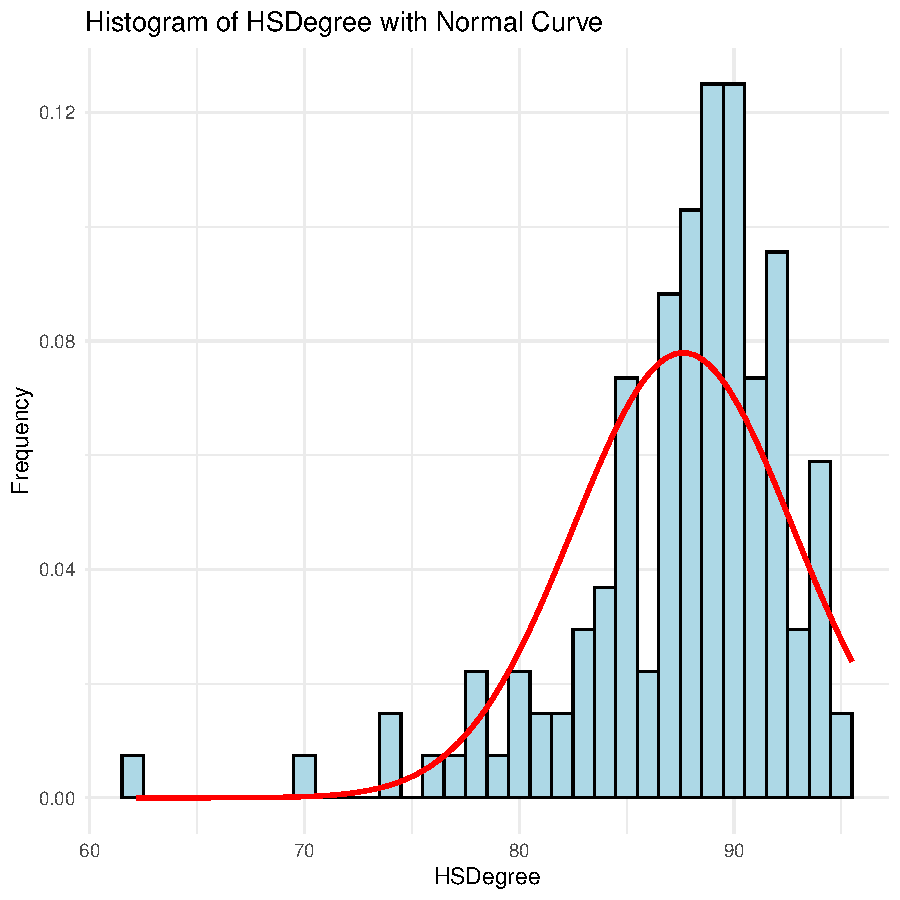
\includegraphics[width=.6\linewidth]{figure/assignment-03-1-Reppeto-Brian-Rnwunnamed-chunk-1-1} 

}


\begin{kframe}\begin{alltt}
\hlcom{## 4.Answer the following questions based on the Histogram produced:}
\hlcom{##    1. Based on what you see in this histogram, is the data }
\hlcom{##        distribution unimodal? ----  Yes the distribution is unimodal.}
\hlcom{##    2. Is it approximately symmetrical? --- No}
\hlcom{##    3. Is it approximately bell-shaped? ----No}
\hlcom{##    4. Is it approximately normal?-----No}
\hlcom{##    5. If not normal, is the distribution skewed? If so, in which direction?}
\end{alltt}
\end{kframe}
\end{knitrout}
\begin{knitrout}
\definecolor{shadecolor}{rgb}{0.969, 0.969, 0.969}\color{fgcolor}\begin{kframe}
\begin{alltt}
\hlcom{##    6. Include a normal curve to the Histogram that you plotted.----Done  }
\hlcom{##    7. Explain whether a normal distribution can accurately be used as a model}
\hlcom{##        for this data.-- T}




\hlcom{## 5. Create a Probability Plot of the HSDegree variable}

\hlkwd{ggplot}\hlstd{(acs_df,} \hlkwd{aes}\hlstd{(}\hlkwc{sample} \hlstd{= HSDegree))} \hlopt{+} \hlkwd{stat_qq}\hlstd{()} \hlopt{+} \hlkwd{stat_qq_line}\hlstd{(}\hlkwc{color}\hlstd{=}\hlstr{"green"}\hlstd{)}
\end{alltt}
\end{kframe}

{\centering 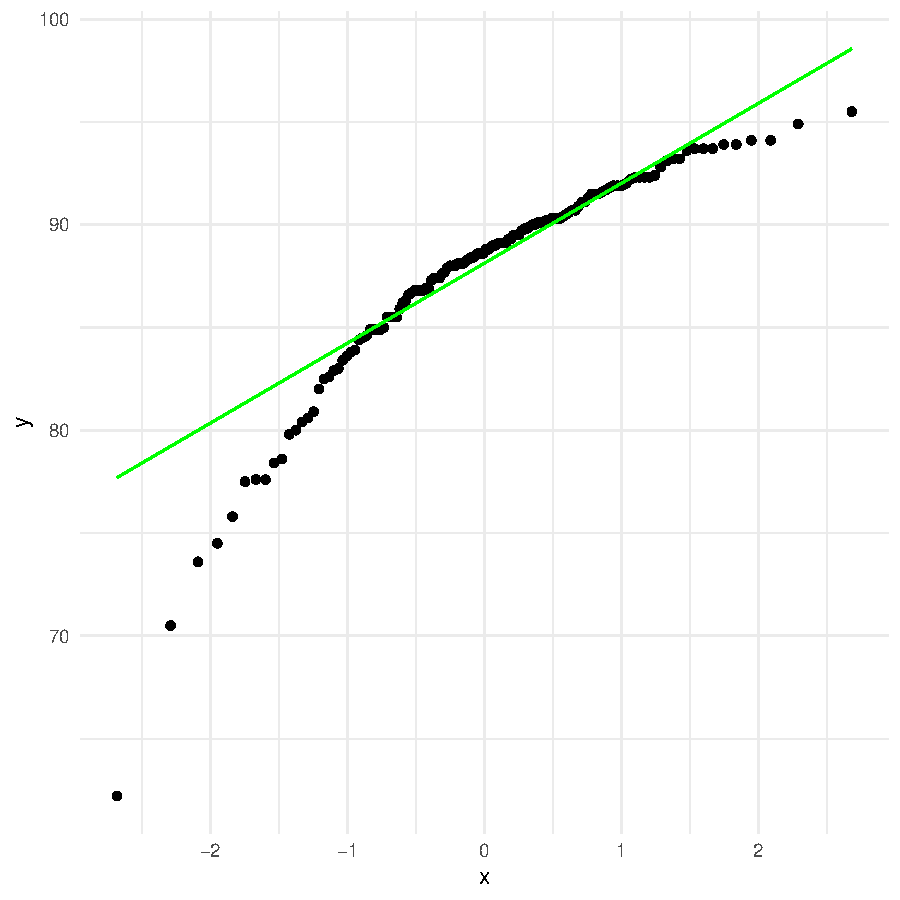
\includegraphics[width=.6\linewidth]{figure/assignment-03-1-Reppeto-Brian-RnwLeft-skewed_unimodal-1} 

}


\begin{kframe}\begin{alltt}
\hlcom{## 6.Answer the following questions based on the Probability Plot:}
\hlcom{##    1.Based on what you see in this probability plot, is the distribution }
\hlcom{##      approximately normal? Explain how you know.--------The distribution is }
\hlcom{##      not normal.  This is based on a normal line test.}
\hlcom{##    2.If not normal, is the distribution skewed? If so, in which direction? }
\hlcom{##      Explain how you know.-------------The plot is left skewed.}




\hlcom{## 7. Now that you have looked at this data visually for normality, you will }
\hlcom{##    now quantify normality with numbers using the stat.desc() function. }
\hlcom{##    Include a screen capture of the results produced.}

\hlkwd{describe}\hlstd{(acs_df}\hlopt{$}\hlstd{HSDegree)}
\end{alltt}
\begin{verbatim}
##    vars   n  mean   sd median trimmed  mad  min  max range  skew kurtosis   se
## X1    1 136 87.63 5.12   88.7   88.28 3.78 62.2 95.5  33.3 -1.67     4.35 0.44
\end{verbatim}
\begin{alltt}
\hlkwd{stat.desc}\hlstd{(acs_df}\hlopt{$}\hlstd{HSDegree,} \hlkwc{basic} \hlstd{=}\hlnum{TRUE}\hlstd{,} \hlkwc{norm} \hlstd{=} \hlnum{FALSE}\hlstd{)}
\end{alltt}
\begin{verbatim}
##      nbr.val     nbr.null       nbr.na          min          max        range 
## 1.360000e+02 0.000000e+00 0.000000e+00 6.220000e+01 9.550000e+01 3.330000e+01 
##          sum       median         mean      SE.mean CI.mean.0.95          var 
## 1.191800e+04 8.870000e+01 8.763235e+01 4.388598e-01 8.679296e-01 2.619332e+01 
##      std.dev     coef.var 
## 5.117941e+00 5.840241e-02
\end{verbatim}
\begin{alltt}
\hlcom{## 8. In several sentences provide an explanation of the result produced for }
\hlcom{##    skew, kurtosis, and z-scores. In addition, explain how a change in the }
\hlcom{##    sample size may change your explanation?}

\hlcom{## Skewness, kurtosis, and z-scores are statistical measures used to analyze the }
\hlcom{## distribution of a dataset. Skewness measures the asymmetry of the data }
\hlcom{## distribution, where positive skewness indicates a longer tail on the }
\hlcom{## right side, negative skewness indicates a longer tail on the left side, }
\hlcom{## and zero skewness represents a symmetric distribution. Kurtosis measures }
\hlcom{## the "tailedness" of the distribution, where positive kurtosis indicates }
\hlcom{## heavier tails and a sharper peak, negative kurtosis indicates lighter tails }
\hlcom{## and a flatter peak, and zero kurtosis represents a normal distribution. }
\hlcom{## Z-scores are a standardized measure that expresses a data point's }
\hlcom{## deviation from the mean in terms of standard deviations.  Since the kurtosis}
\hlcom{## is greater than 3 this indicates the leptokurtic has lang and skinny tails}
\hlcom{## this means there are more chances of outliers.  Additionally, the negative}
\hlcom{## skew indicates the data points are more concentrated towards the right}
\hlcom{## side of the distribution, and makes the mean bend more toward the right also.}
\hlcom{## A change in the sample size can affect the interpretation of these measures. }
\hlcom{## Skewness and kurtosis are influenced by extreme values, and as the sample }
\hlcom{## size increases, the impact of outliers or extreme values tends to diminish. }
\hlcom{##  Therefore, larger sample sizes may result in more accurate estimates of }
\hlcom{## skewness and kurtosis, providing a better representation of the underlying }
\hlcom{## population. On the other hand, z-scores are not directly affected by sample }
\hlcom{## size since they are calculated based on the mean and standard deviation. }
\hlcom{## However, a larger sample size can provide more reliable estimates of the }
\hlcom{## mean and standard deviation, leading to more precise z-scores.}
\end{alltt}
\end{kframe}
\end{knitrout}

The R session information (including the OS info, R version and all
packages used):

\begin{knitrout}
\definecolor{shadecolor}{rgb}{0.969, 0.969, 0.969}\color{fgcolor}\begin{kframe}
\begin{alltt}
\hlkwd{sessionInfo}\hlstd{()}
\end{alltt}
\begin{verbatim}
## R version 4.3.0 (2023-04-21)
## Platform: aarch64-apple-darwin20 (64-bit)
## Running under: macOS Ventura 13.4
## 
## Matrix products: default
## BLAS:   /System/Library/Frameworks/Accelerate.framework/Versions/A/Frameworks/vecLib.framework/Versions/A/libBLAS.dylib 
## LAPACK: /Library/Frameworks/R.framework/Versions/4.3-arm64/Resources/lib/libRlapack.dylib;  LAPACK version 3.11.0
## 
## locale:
## [1] en_US.UTF-8/en_US.UTF-8/en_US.UTF-8/C/en_US.UTF-8/en_US.UTF-8
## 
## time zone: America/Chicago
## tzcode source: internal
## 
## attached base packages:
## [1] stats     graphics  grDevices utils     datasets  methods   base     
## 
## other attached packages:
## [1] pastecs_1.3.21 psych_2.3.6    ggplot2_3.4.2 
## 
## loaded via a namespace (and not attached):
##  [1] crayon_1.5.2     vctrs_0.6.3      knitr_1.43       nlme_3.1-162     cli_3.6.1       
##  [6] xfun_0.39        rlang_1.1.1      highr_0.10       generics_0.1.3   glue_1.6.2      
## [11] labeling_0.4.2   colorspace_2.1-0 scales_1.2.1     fansi_1.0.4      grid_4.3.0      
## [16] evaluate_0.21    munsell_0.5.0    tibble_3.2.1     lifecycle_1.0.3  compiler_4.3.0  
## [21] dplyr_1.1.2      pkgconfig_2.0.3  rstudioapi_0.14  lattice_0.21-8   farver_2.1.1    
## [26] R6_2.5.1         tidyselect_1.2.0 utf8_1.2.3       pillar_1.9.0     mnormt_2.1.1    
## [31] parallel_4.3.0   magrittr_2.0.3   tools_4.3.0      withr_2.5.0      gtable_0.3.3    
## [36] boot_1.3-28.1
\end{verbatim}
\begin{alltt}
\hlkwd{Sys.time}\hlstd{()}
\end{alltt}
\begin{verbatim}
## [1] "2023-06-24 21:07:42 CDT"
\end{verbatim}
\end{kframe}
\end{knitrout}


\end{document}
